\documentclass{article}
\usepackage[utf8]{inputenc}
\usepackage[T1]{fontenc}
\usepackage{graphicx}
\begin{document}
\newlength{\picwidth}
\setlength{\picwidth}{2.5cm}
\begin{description}
\item[Rodrigo C.\,M.~Santos] Rodrigo has Bachelor’s Degree (2010) and
  Master’s Degree (2013) in Computer Science from Federal University of
  Maranhão, where he worked as a researcher for the Laboratory of Advanced
  Web Systems (LAWS Lab). In 2013, he joined the TeleMídia Lab. of PUC-Rio,
  working on the evolution and maintenance of the Ginga-NCL middleware and
  related tools.  From 2016 to 2018, he was a Research Software Engineering
  intern at IBM Research Brazil. Currently, Rodrigo is a Research Software
  Engineer at IBM Research Brazil, where he works mainly with knowledge
  engineering and AI.
  % \begin{center}
  %   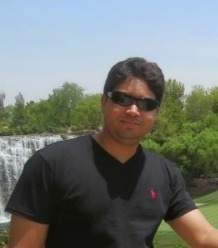
\includegraphics[width=\picwidth]{pics/rodrigo.jpg}
  % \end{center}

\item[Guilherme F.~Lima] Holds a DSc (2015) and a MSc (2011) in Informatics
  and a BA (2008) in Information Systems, all from PUC-Rio, Brazil.  His
  research interests are in languages and models for synchronous programming
  and multimedia, and in formal methods applied to computer programming in
  general.
  % \begin{center}
  %   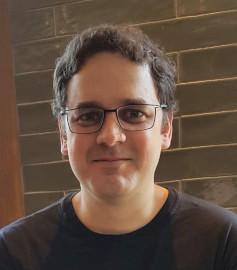
\includegraphics[width=\picwidth]{pics/guilherme.jpg}
  % \end{center}

\item[Francisco Sant'Anna] Francisco is an Adjunct Professor of Computer
  Science at UERJ.  He holds a D.Sc. in Computer Science from PUC-Rio.  His
  interests are in programming languages and concurrent systems.  Currently,
  he develops the programming language Céu, exploring the synchronous and
  reactive approach to concurrent programming.
  % \begin{center}
  %   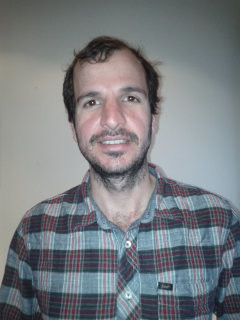
\includegraphics[width=\picwidth]{pics/francisco.jpg}
  % \end{center}

\item[Roberto Ierusalimschy] Roberto is the leading architect of the Lua
  programming language, driving its development since its inception in
  1993. He is an Associate Professor of Computer Science at PUC-Rio (the
  Pontifical Catholic University of Rio de Janeiro), where he works with
  programming-language design and implementation.
  %%
  Roberto has a M.Sc. Degree and a D.Sc. Degree in Computer Science, both
  from PUC-Rio. He was a visiting researcher at the University of Waterloo,
  ICSI, GMD, and UIUC, and a Tinker Professor at Stanford. As a professor at
  PUC-Rio, Roberto was the advisor of several students that later became
  influential members of the Lua community. Roberto is also a Distinguished
  ACM Speaker and a member of the IFIP Working Group on Language Design.
  % \begin{center}
  %   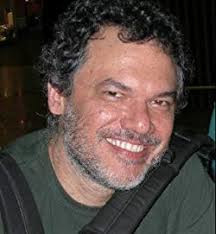
\includegraphics[width=\picwidth]{pics/roberto.jpg}
  % \end{center}

\item[Edward Hermann Haeusler] Edward Hermann Haeusler has a Bachelor's
  Degree in Mathematics from UnB (1983), and a M.Sc. Degree (1986) and a
  D.Sc. Degree (1990) in Informatics, both from PUC-Rio.  Currently, he is
  an Associate Professor at PUC-Rio.  His research interests are in
  computability and models of computation with emphasis on proof theory,
  category theory, formal semantics, and logic.
  % \begin{center}
  %   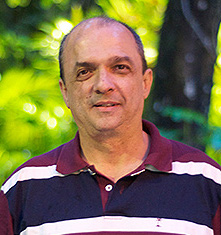
\includegraphics[width=\picwidth]{pics/hermann.jpg}
  % \end{center}
\end{description}
\end{document}

%%% Local Variables:
%%% mode: latex
%%% TeX-master: t
%%% End:
